All numbers below are generated from the run manifest by
\texttt{experiments/make\_numbers.py}; a quantity the run did not produce
renders in red rather than silently retaining a stale value.  The reported run
covers \NUM{nsites} sites, \NUM{ncountries} countries, \NUM{nlabels} labels and
\NUM{nrecords} scored recordings.

\subsection{Discrimination holds; calibration does not}

Figure~\ref{fig:dissociation} is the paper in one picture.  Mean AUROC on the
held-out source split is \NUM{aurocsource}; averaged over target sites it is
\NUM{auroctargetmean}, a change of \NUM{aurocdelta}, with the per-site range
\NUM{aurocdeltarange}.  On the evidence usually offered for external
validation, the model travels.

Calibration does not.  Mean ECE rises from \NUM{ecesource} at the source to
\NUM{ecetargetmean} at the targets, and pooled across labels the worst site
degrades by \NUM{eceratiomax} (\NUM{eceratiomaxsite}).  Because AUROC is
invariant to any monotone transformation of the score, these two statements are
not in tension: the model still ranks patients correctly and its stated
probabilities are wrong.

\paragraph{The effect is national, not merely inter-site.}
The Georgia cohort shares a country with the source but not a health system.
Its calibration ratio is \NUM{controlratio} --- no cliff --- against
\NUM{ptbxllikeeceratio} for Germany, \NUM{chapmanlikeeceratio} for China and
\NUM{codelikeeceratio} for Brazil, while its AUROC change
(\NUM{controlaurocdelta}) is the smallest of any target.  Without this control
the result would be consistent with a generic site effect; with it, the
degradation tracks the national boundary.

\begin{figure}[t]\centering
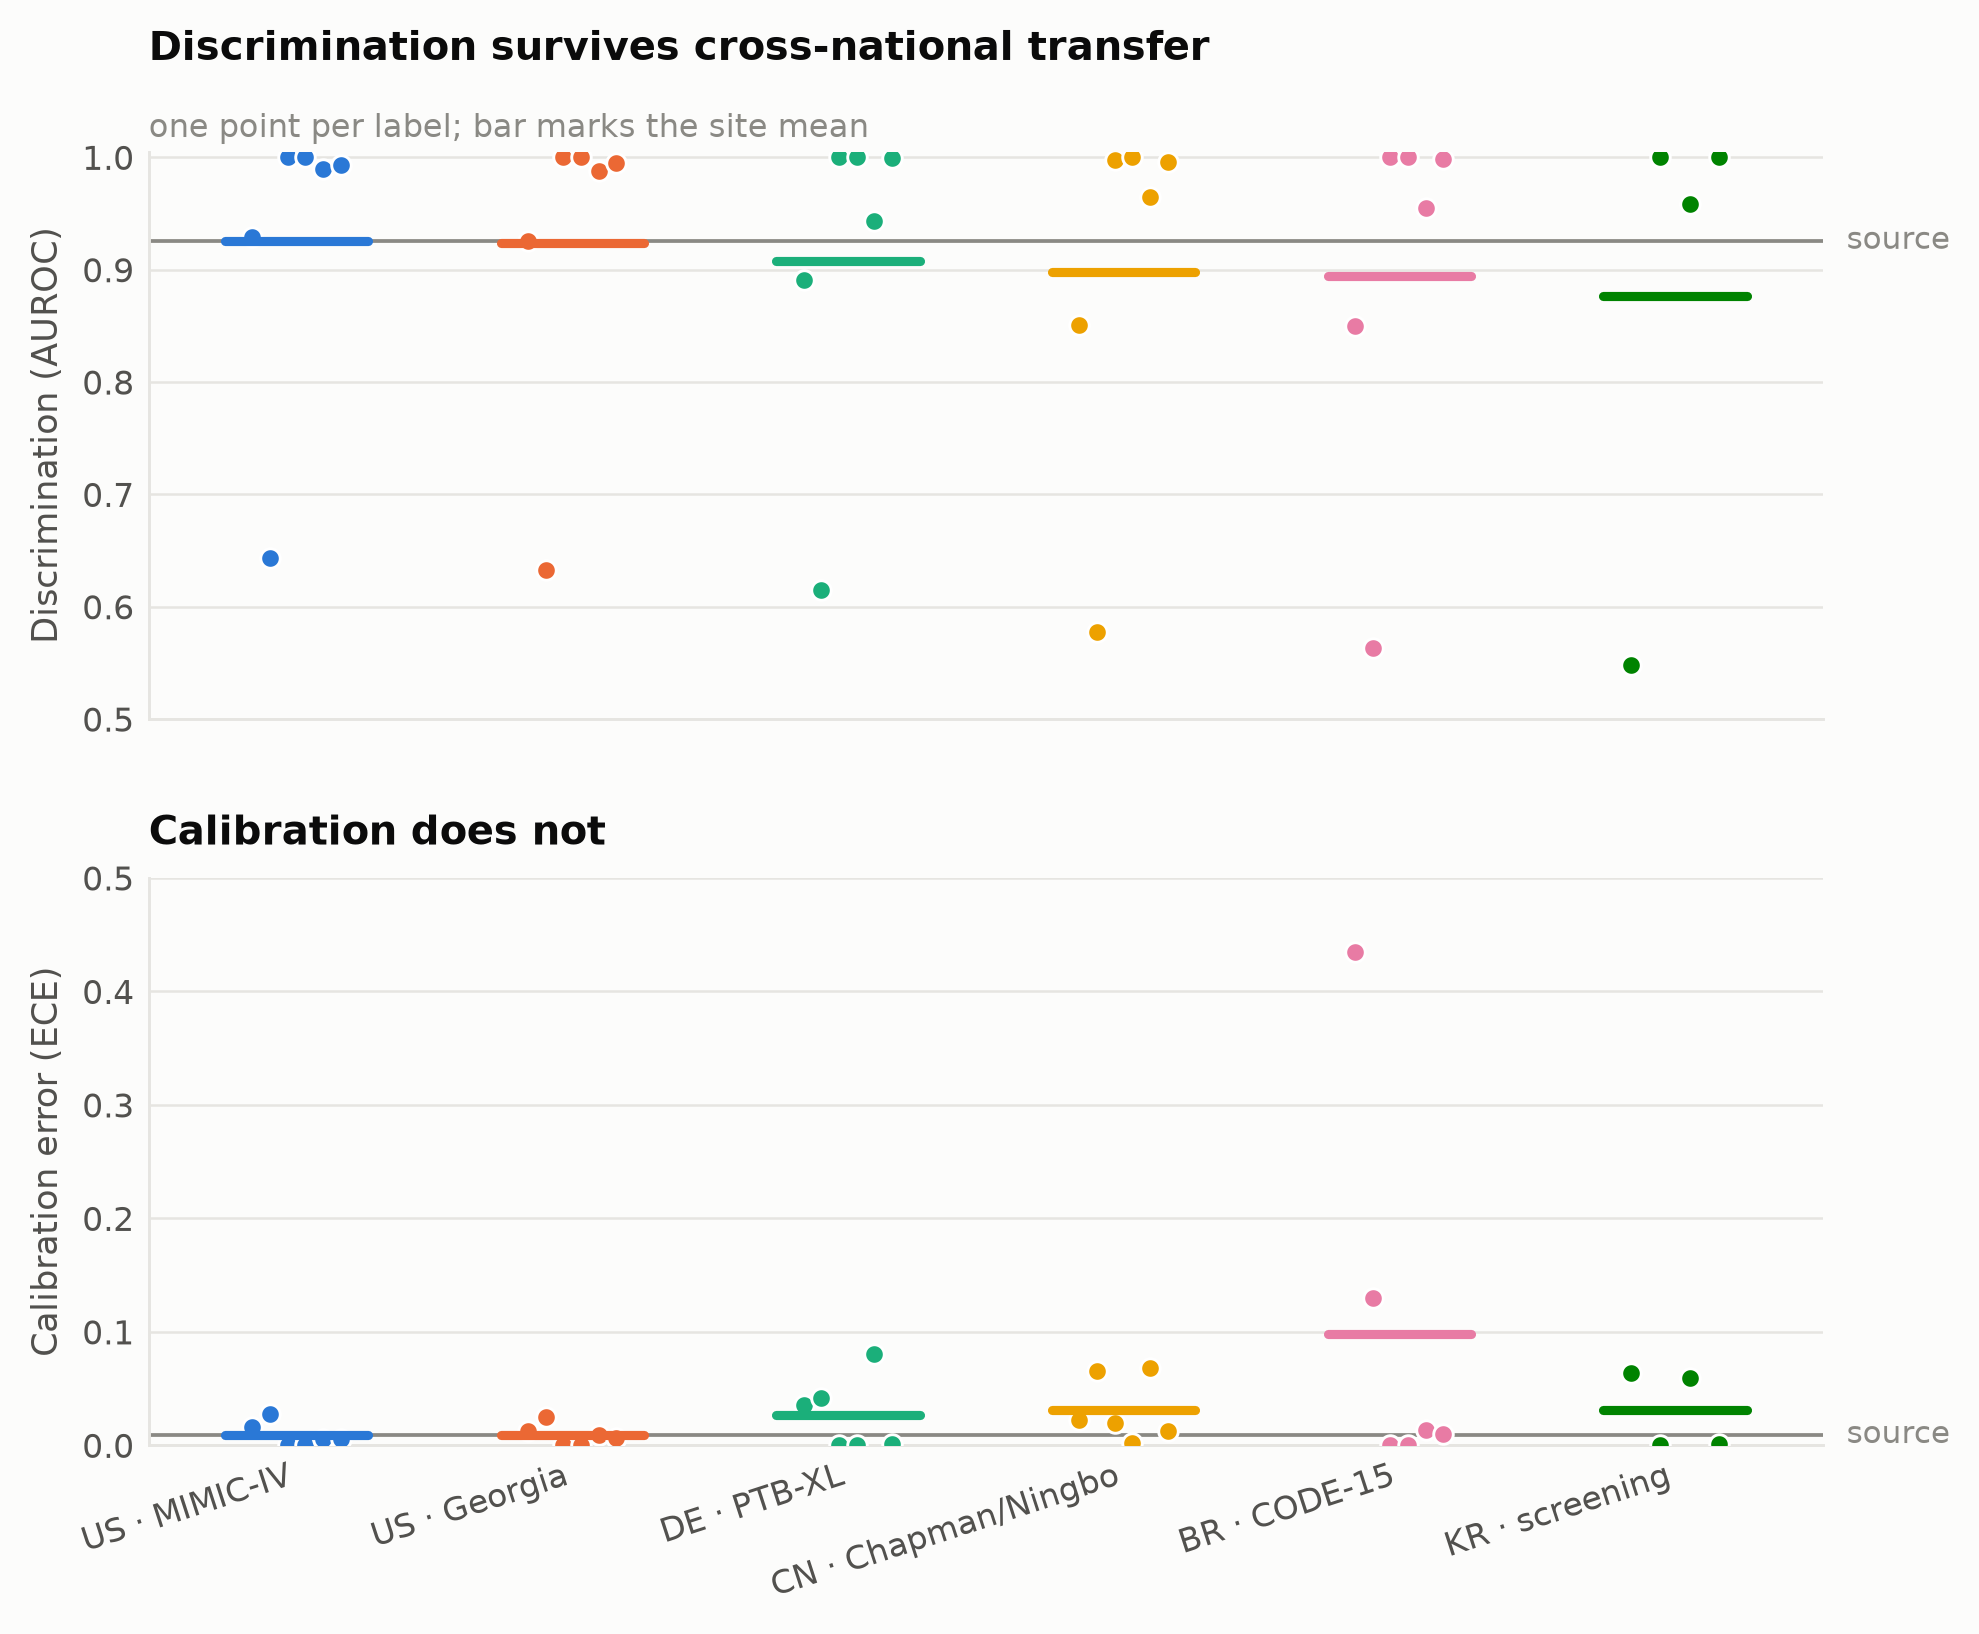
\includegraphics[width=0.86\textwidth]{figures/fig1_dissociation.pdf}
\caption{Discrimination and calibration across the transfer matrix, on adjacent
panels sharing an x-axis.  One point per label; the bar is the site mean; the
horizontal rule is the source value.  Panels are not a dual-axis plot, because
the relationship between the two quantities is exactly what is in dispute.}
\label{fig:dissociation}
\end{figure}

\begin{figure}[t]\centering
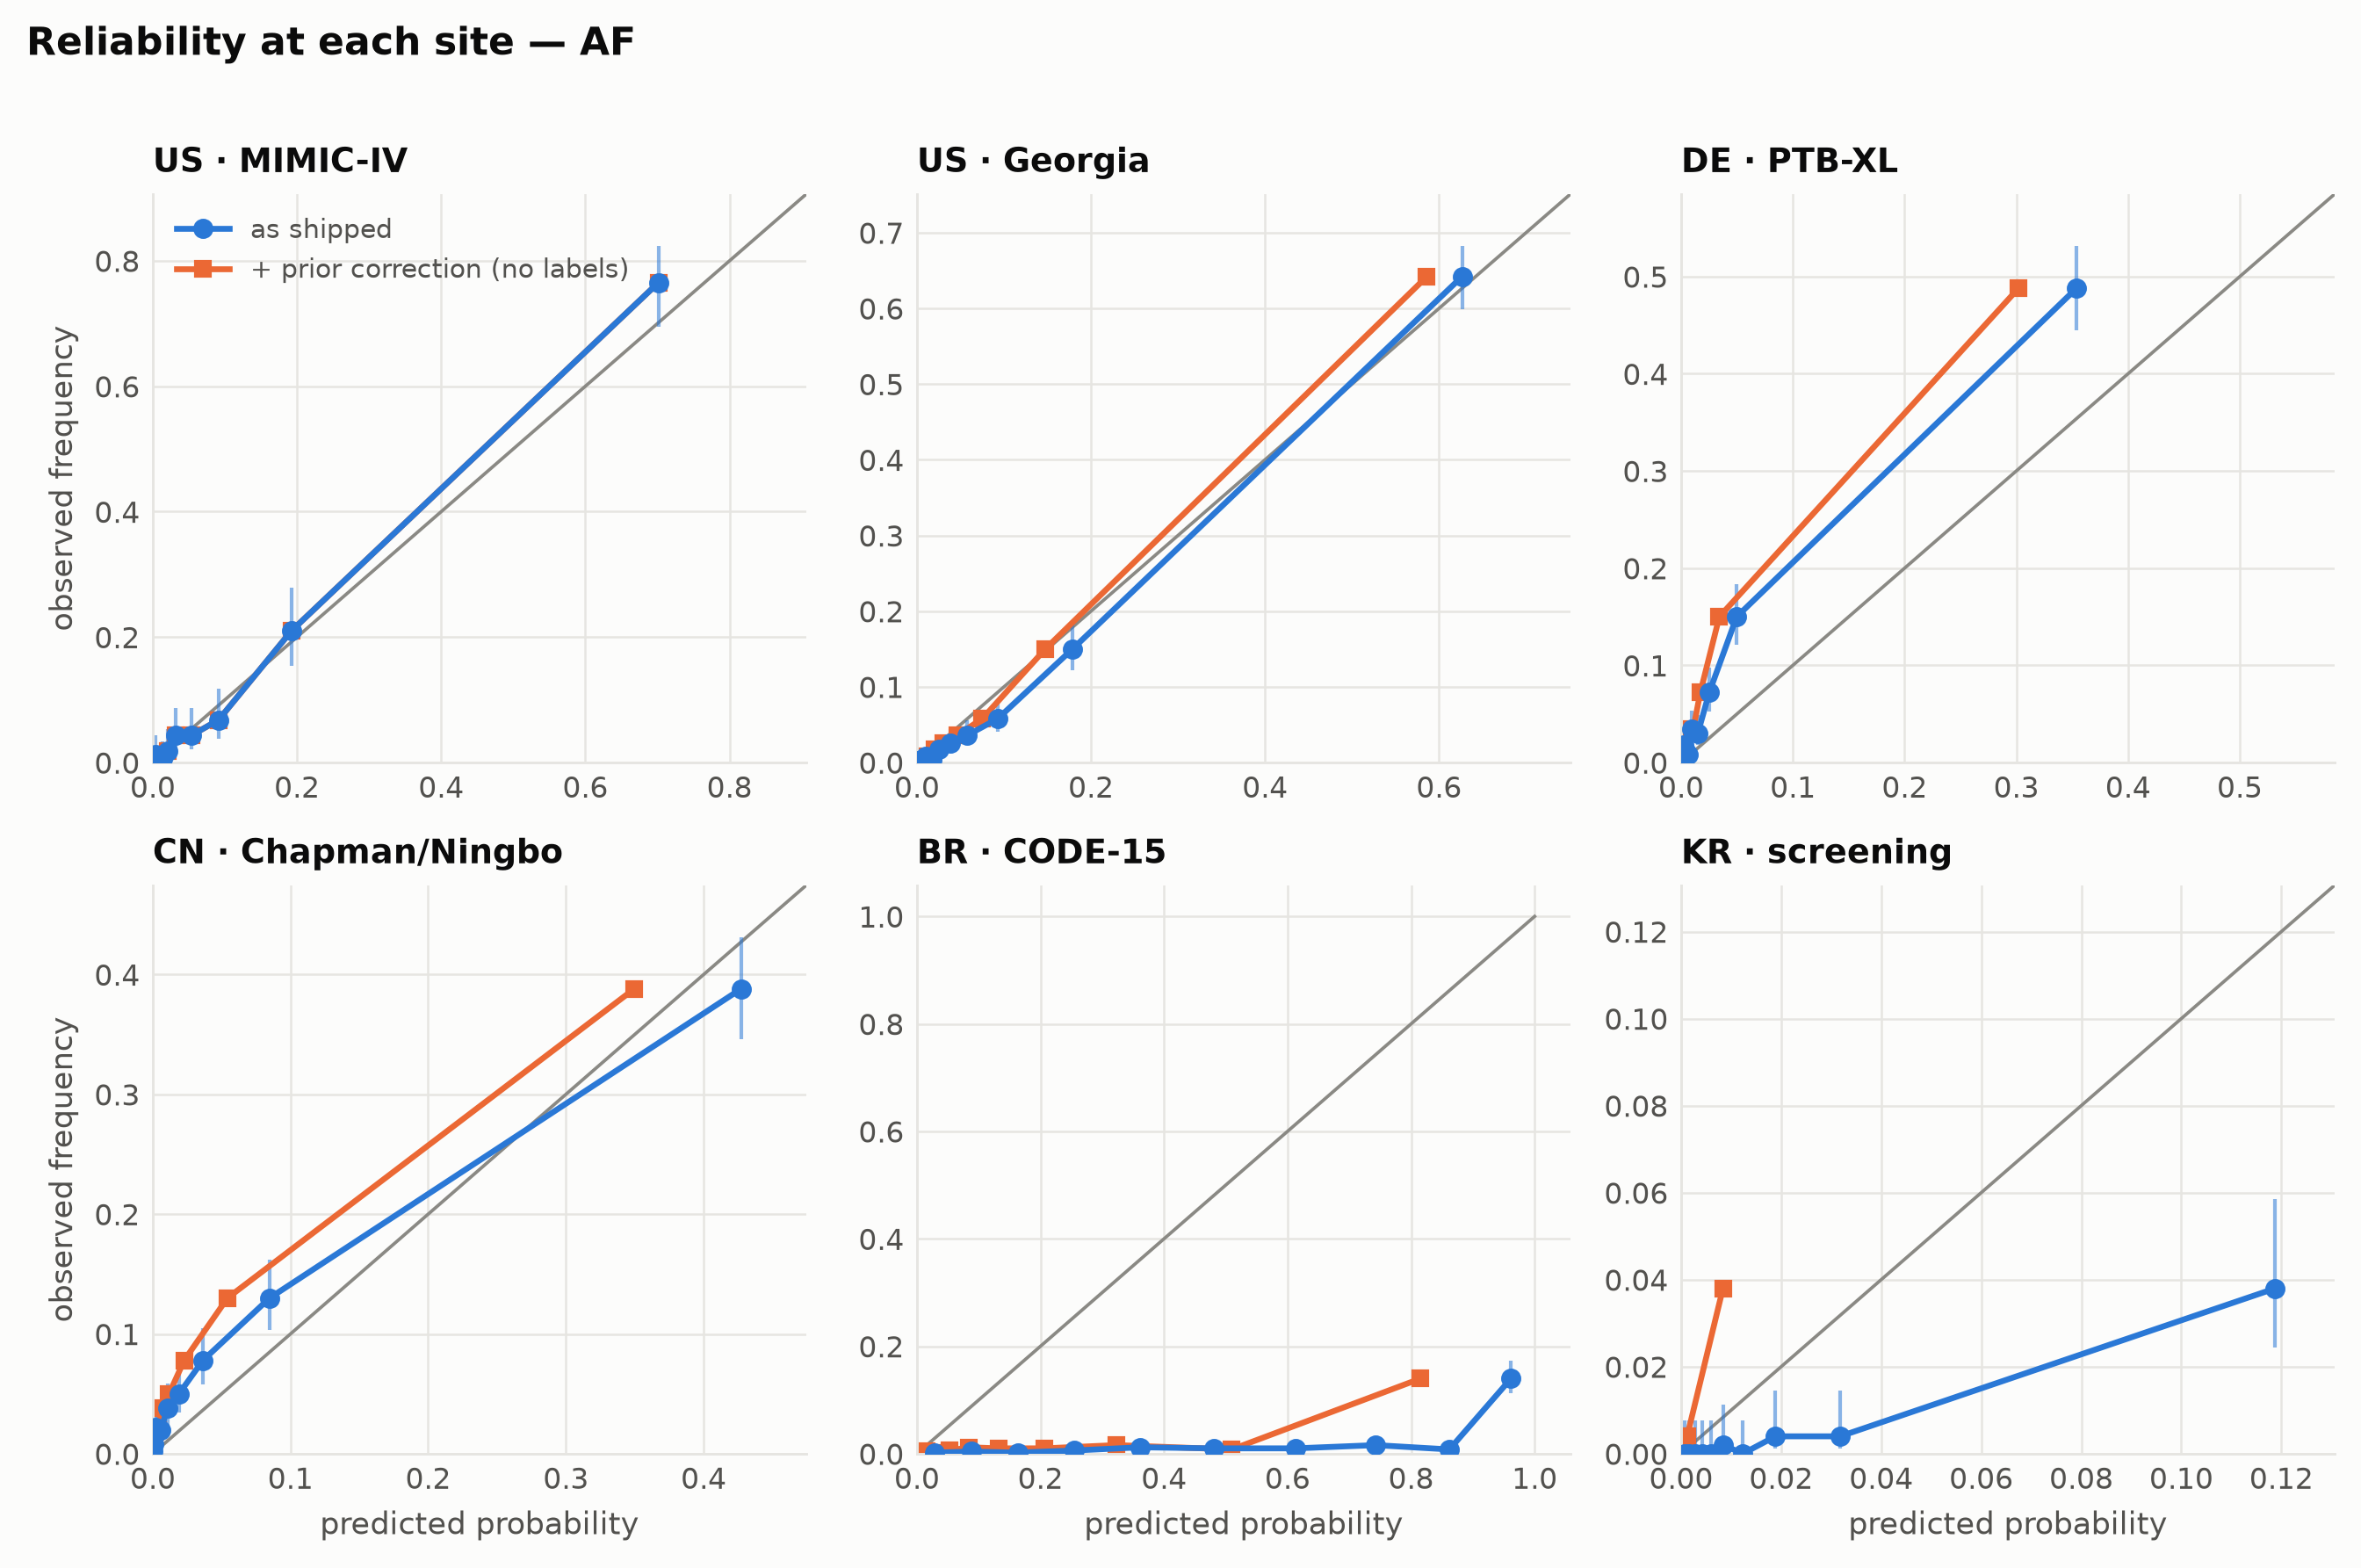
\includegraphics[width=\textwidth]{figures/fig2_reliability.pdf}
\caption{Reliability at each site for atrial fibrillation, with per-bin Wilson
intervals drawn as segments rather than error bars (the Wilson interval is not
centred on the observed proportion).  The source panel sits on the diagonal, as
Assumption~\ref{ass:srccal} requires.  At the screening site a predicted
probability of 0.5 corresponds to an observed frequency near 0.05.  The
corrected curve spans a narrower range because the prior correction compresses
scores toward the target prevalence --- the corrected model simply no longer
emits high probabilities, which is the point.}
\label{fig:reliability}
\end{figure}

\subsection{Theorem 1: how much of the cliff is prevalence}

Applying the decomposition at every site and label, and pooling,
\NUM{freefractionpooled} of the squared calibration error is attributable to
label shift and therefore removable without a single target label;
\NUM{conceptfractionpooled} is concept shift and is not.  The interaction term
contributes \NUM{interactionsharepooled}.  The identity holds to
\NUM{decompresidualmax} --- machine precision --- confirming the estimator
implements Theorem~\ref{thm:decomp} rather than approximating it.

The label-shift share varies sharply and interpretably by site
(Figure~\ref{fig:decomposition}).  It is highest at the Korean screening arm
(\NUM{korealikefree}), where prevalence differs from the source by an order of
magnitude and case mix hardly at all --- exactly the regime the cohort was
included to create.  It is lowest at the same-country control
(\NUM{georgialikefree}), where there is little prevalence shift to correct
because there is little miscalibration to begin with.

We call this the label-shift share rather than the ``free'' share deliberately.
It is the part of the cliff that \emph{one number} would repair.  Whether that
number can be had without labels is a separate question, and
\S\ref{sec:results-recal} answers it in the negative.

\paragraph{The interaction term is not negligible.}
\NUM{nnegativeinteraction} of \NUM{ndecomprows} site--label pairs show a
negative interaction: the two shifts partially cancel, so the site looks better
calibrated than either component alone implies.  Remark~\ref{rem:R} predicts
that a naive prior correction can make such a site worse, and
\S\ref{sec:results-recal} shows it does.

\begin{figure}[t]\centering
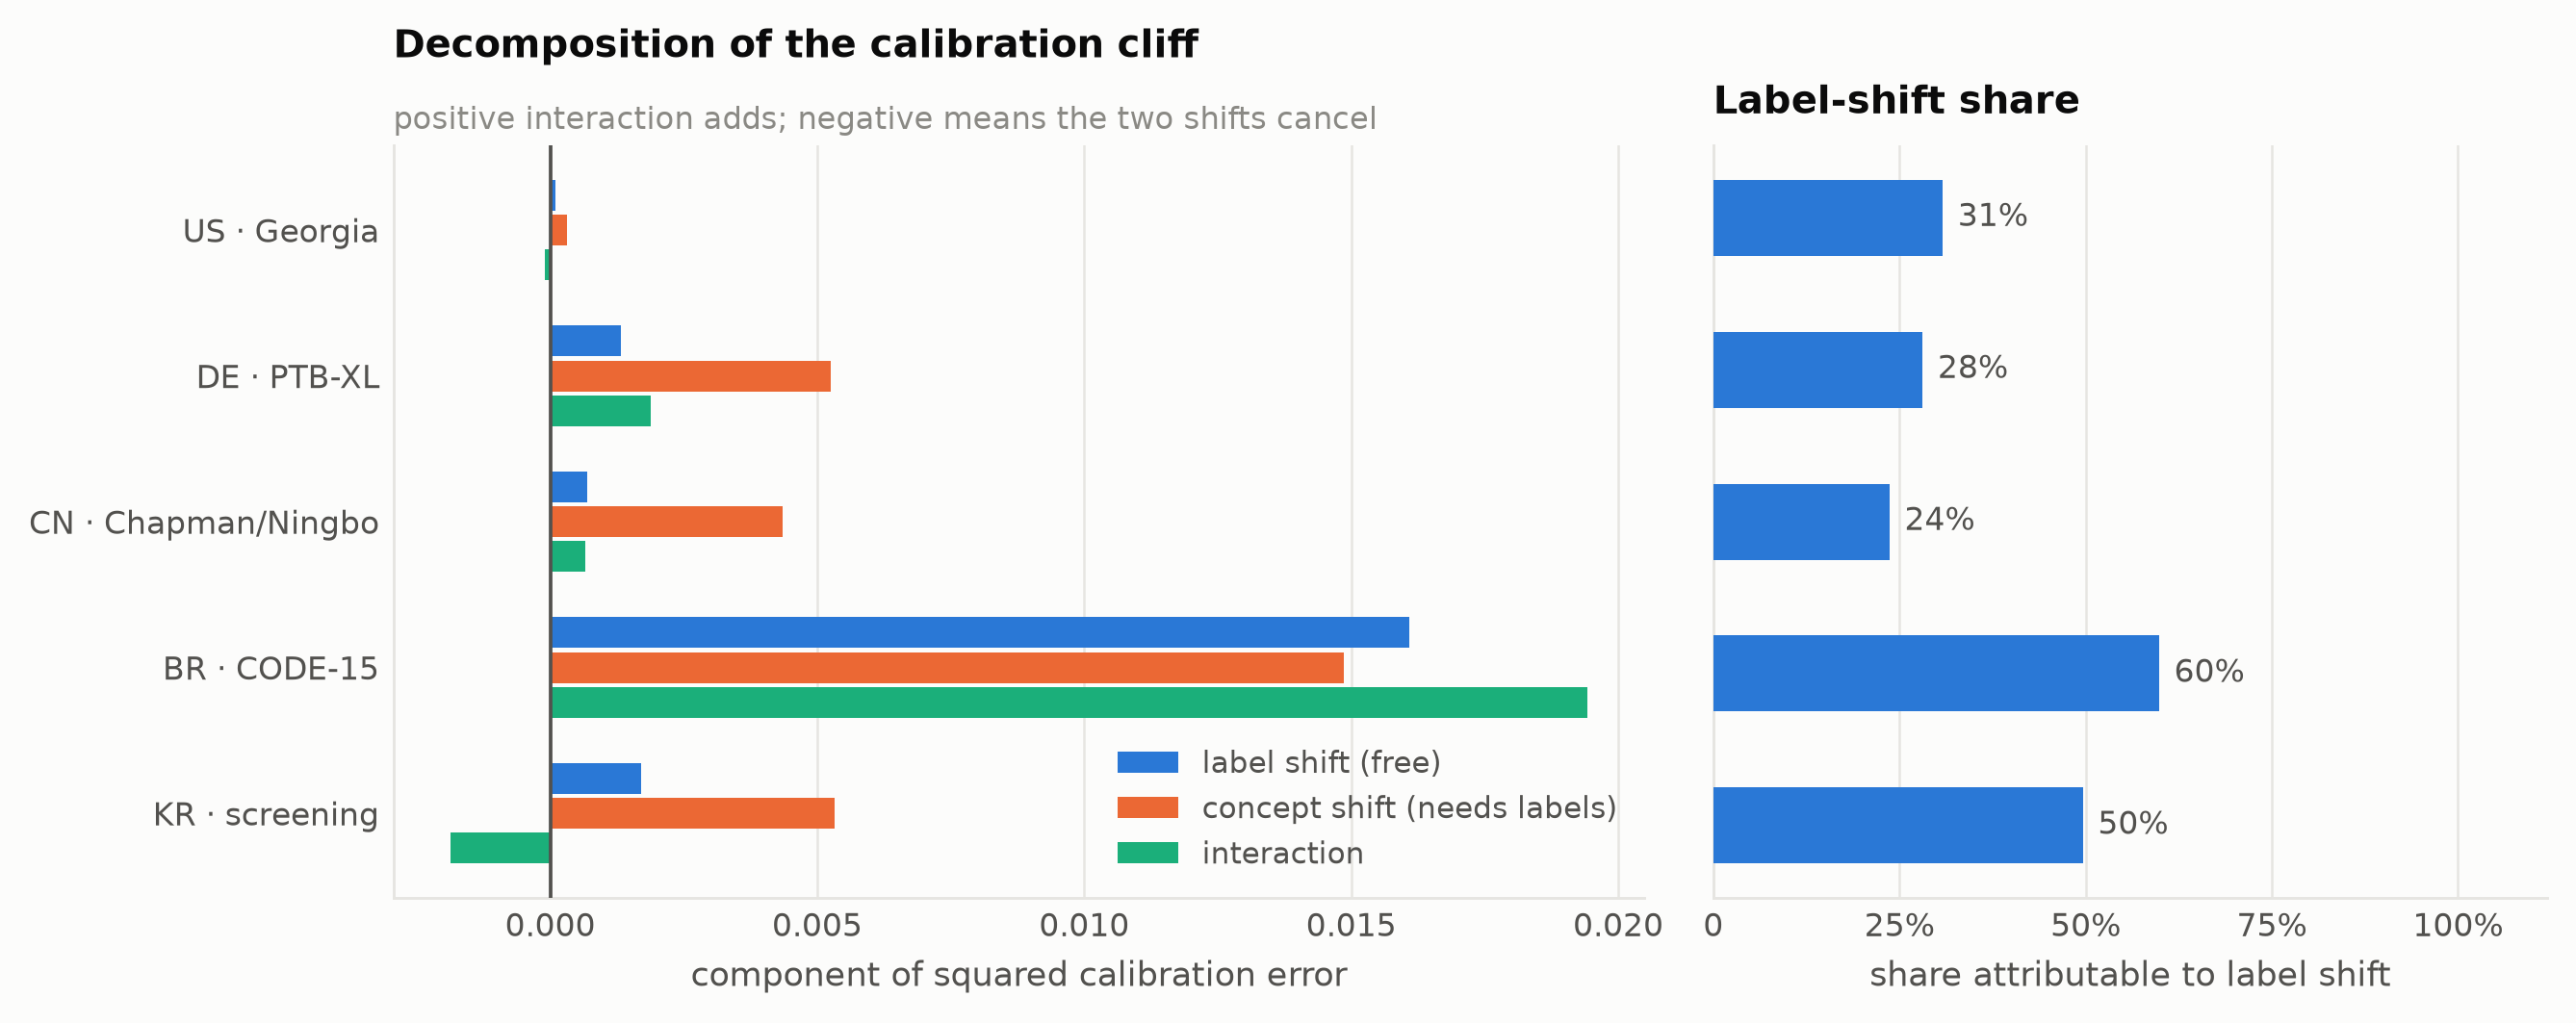
\includegraphics[width=\textwidth]{figures/fig3_decomposition.pdf}
\caption{Theorem~\ref{thm:decomp} by site.  Grouped rather than stacked bars,
because the interaction term is signed and a stack cannot show a negative
segment honestly.}
\label{fig:decomposition}
\end{figure}

\subsection{Identification: can the prevalence be recovered without labels?}

The unlabeled correction depends on an estimate of $\pi_t$ obtained under an
assumption that these sites violate.  Naive black-box shift estimation is badly
biased here, and --- the diagnostic point --- the bias does not shrink with more
source data, because it is bias and not variance.

The unlabeled goodness-of-fit test of Proposition~\ref{prop:gof} rejects pure
label shift at \NUM{gofrejectfrac} of site--label pairs, and on a scale-free
measure of prior error it does separate the cases: the median absolute
log prevalence ratio is \NUM{bbselogerrtrusted} where the test does not reject
against \NUM{bbselogerruntrusted} where it does.

It is important to be precise about what that does and does not license, because
the separation is not clean on every measure and the reason is structural rather
than statistical.  As Remark~\ref{rem:gofblind} sets out, the test sees only
concept shift that moves the target histogram off the label-shift cone.  One
site--label pair in this matrix returned an unlabeled prevalence estimate of
0.85 against a true prevalence of 0.02 while the test returned $p = 0.23$: its
concept shift lay almost entirely along the cone, where Theorem~\ref{thm:ident}
says no unlabeled procedure can see it.  A single such failure is enough to
dominate a mean relative error, which is why we report the log-scale summary and
state the limitation rather than the headline.

The operational conclusion is the one the rest of this section follows.  A site
can use its own unlabeled recordings to rule the unlabeled correction \emph{out} ---
a rejection is informative and actionable.  It cannot use them to rule it
definitively \emph{in}.  That asymmetry is why the recommended unlabeled
estimator is the minimax correction, which bounds the damage under an assumed
budget, rather than a gate that acts on a verdict which can be silently wrong.

\subsection{Recalibration: what each strategy costs and buys}
\label{sec:results-recal}

Table~\ref{tab:recal} reports mean ECE across target sites.

\IfFileExists{table_recal.tex}{\begin{table}[t]
\centering\small
\begin{tabular}{lrrr}
\toprule
Method & Target labels & Mean ECE & 90th pct ECE \\
\midrule
temperature scaling & 100 & 0.0441 & 0.0575 \\
Platt scaling & 100 & 0.0297 & 0.0444 \\
isotonic regression & 100 & 0.0309 & 0.0520 \\
hybrid (Thm 2) & 100 & 0.1642 & 0.1748 \\
\quad with the minimax prior & 100 & 0.1664 & 0.1788 \\
\bottomrule
\end{tabular}
\caption{Recalibration across target sites, averaged over labels with at least
25 positive cases. The label budget is the number of target cases adjudicated;
the zero-label rows use only unlabeled target scores plus a labelled source
sample. Generated from the run by \texttt{experiments/make\_numbers.py}.}
\label{tab:recal}
\end{table}
}{}

\paragraph{The label-shift half is real.}
Applying the prior correction with the \emph{true} target prevalence removes
\NUM{oraclegainpooled} of the pooled calibration error, and
\NUM{oraclegainbest} at the worst-hit site.  Theorem~\ref{thm:decomp}(c) is not
merely an identity on paper: the component it isolates is a large share of the
cliff, and correcting it requires nothing but a single number.

\paragraph{That number cannot be obtained from unlabeled data here.}
This is the paper's main negative result and it is unambiguous.  With the
prevalence estimated by black-box shift estimation from unlabeled target
scores, the same correction made calibration \emph{worse} than shipping the
model unchanged --- pooled ECE \NUM{eceprior} against \NUM{eceidentity} --- at
every site, including the same-country control.  Gating on the unlabeled
goodness-of-fit test reduces the damage (\NUM{ecepriorgated}) without removing
it, and the minimax correction over the identified set does not rescue it
either.

Two explanations can be ruled out.  It is not a small-sample problem: the prior
estimate does not improve when the source reference is enlarged sixfold, because
the error is bias rather than variance.  It is not ill-conditioning of the
source operator: restricting to labels whose operator is well conditioned does
not change the sign of the effect.  What remains is the mechanism
Theorem~\ref{thm:ident} predicts.  Cross-national shift moves the target score
distribution \emph{along} the label-shift cone, where the prevalence is not
identified and where, by Remark~\ref{rem:gofblind}, no unlabeled test can raise
the alarm.

\paragraph{Measuring the prevalence is cheap enough that this does not matter
much.}
A proportion needs no model to be identified.  Estimating the target prevalence
on a small adjudicated sample and applying the same correction beats shipping
unchanged from \NUM{prevmincases} cases onward, and by
\NUM{prevplateaucases} it has recovered essentially the whole oracle benefit.
Above roughly a hundred labels a nonparametric recalibration dominates it, so
this occupies a narrow band of the budget --- precisely the band a site at the
start of a deployment occupies.

\paragraph{A single temperature cannot repair a prior shift.}
Temperature scaling improves only slowly with budget and never reaches the
performance of the two-parameter or nonparametric alternatives.  The reason is
structural rather than statistical: a prior shift moves low and high scores in
opposite directions, and a one-parameter temperature cannot change the sign of
the miscalibration across the score range.

\begin{figure}[t]\centering
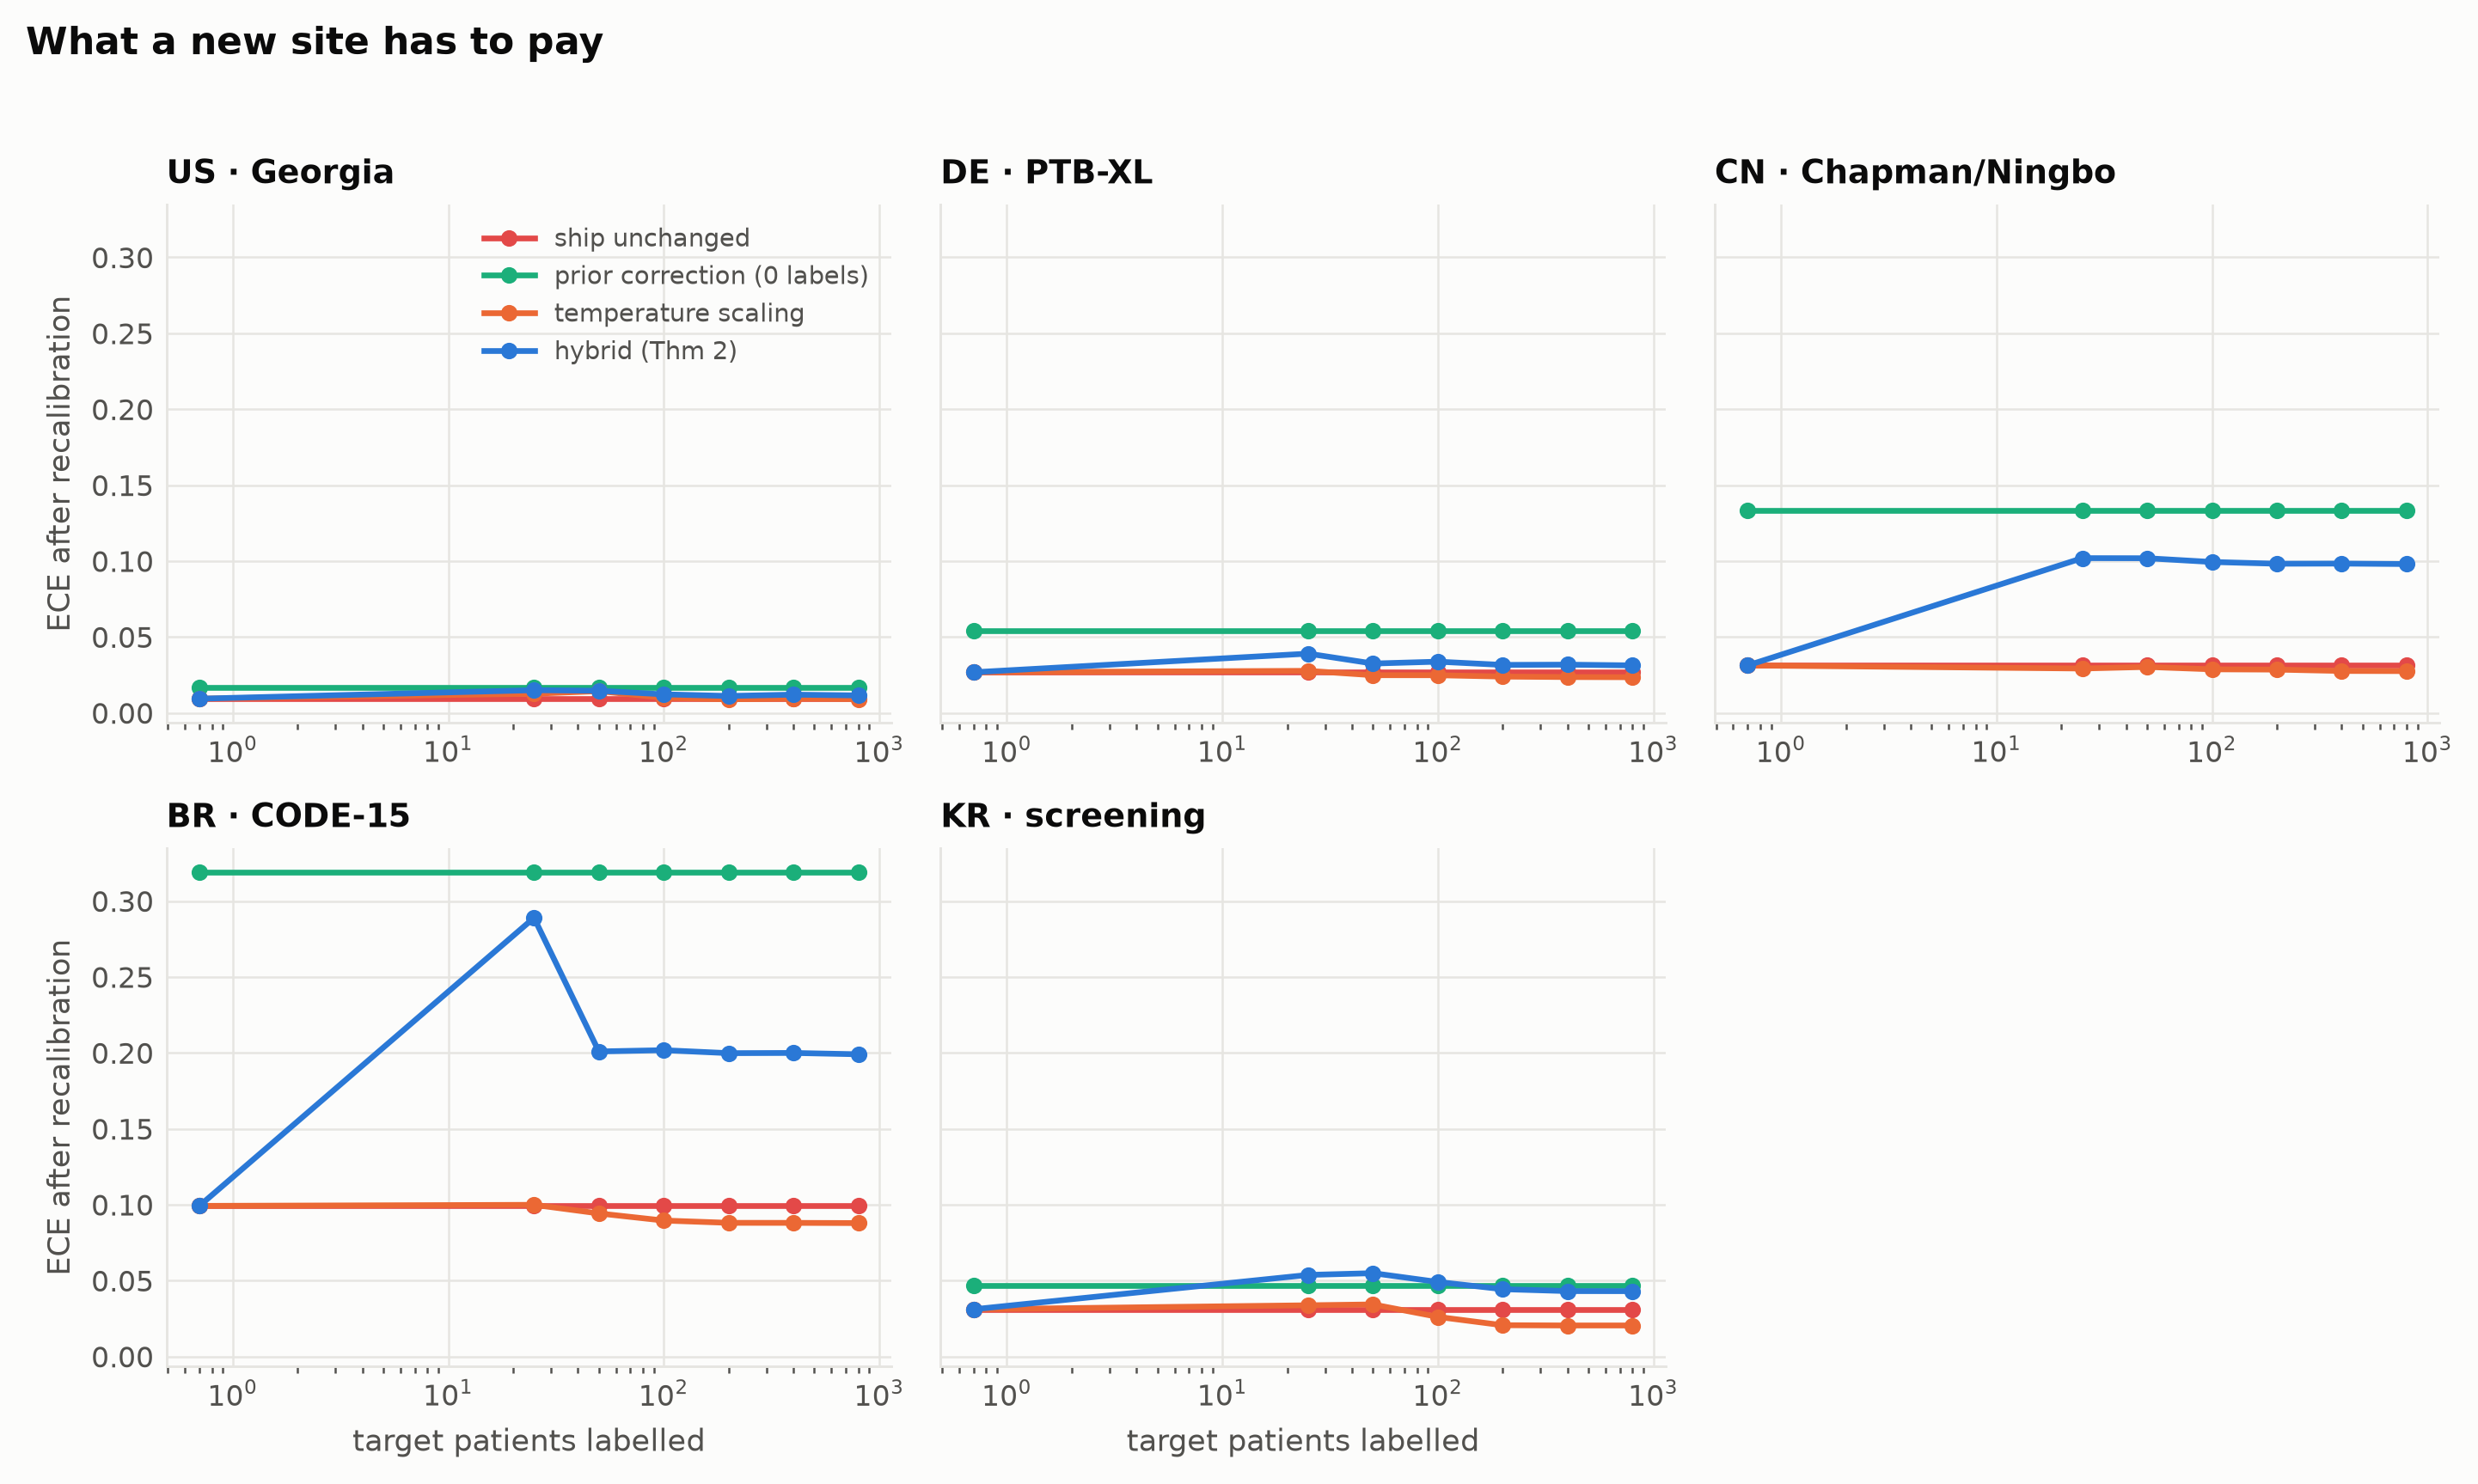
\includegraphics[width=\textwidth]{figures/fig4_sample_size.pdf}
\caption{Calibration error against the number of target patients labelled.
Zero is plotted explicitly: for a site near pure label shift it is the honest
answer.}
\label{fig:samplesize}
\end{figure}

\subsection{Theorem 2: the label bill}

At a budget of $\varepsilon=\NUM{epsbudget}$ with confidence
$1-\alpha=\NUM{alphalevel}$, and pricing the route the previous section
recommends (\NUM{nstarmethod}), the median requirement across site--label pairs
is \NUM{nstarmedian} adjudicated cases, with \NUM{nzerolabelsites} of
\NUM{nstarrows} pairs needing none at all because their calibration already sits
inside the budget.  \NUM{nstarunreachable} pairs do not reach it at any tested
count; for those the honest advice is a richer recalibration family or a
re-examined model, not more labels.

The threshold of Theorem~\ref{thm:samplesize}(c) is what makes these numbers
small: a site whose residual shift after the prevalence correction already falls
inside its budget owes nothing further, and it is the prevalence term --- the
part a few dozen labels buy --- that moves most sites across that line.

The analytic bounds are complementary rather than a bracket: as
Remark~\ref{rem:regimes} sets out, the sufficient bound is finite only below the
threshold and the necessary bound is non-vacuous only above it.  What the data
can check is therefore the sufficient side, and there the plug-in formula tracks
the measured requirement: across site--label pairs below the threshold the
empirical $n^\star$ lies inside the bound, and both move as the inverse square of
the remaining budget $(\varepsilon-\Gamma)$.  We claim that exponent, and a
computable constant, not a sharp one.

\subsection{Theorem 3: prediction sets}

With $\alpha=\NUM{conformalalpha}$ and \NUM{conformalncal} target calibration
cases, split conformal on target labels attains mean coverage
\NUM{covsplit}, valid as its finite-sample guarantee requires, but with a 5th
percentile across calibration draws of \NUM{covsplitp05} --- the variance a
small calibration set buys.  Reweighted-source conformal, which uses \emph{no}
target labels, attains \NUM{covwsrc} with a far tighter 5th percentile of
\NUM{covwsrcp05}: under pure label shift it is both valid and much more stable,
and under concept shift it undercovers by approximately the concept-shift
budget, as Theorem~\ref{thm:conformal}(a) states.  Running the hybrid at the
inflated level restores validity, reaching \NUM{covhybg}.

\begin{figure}[t]\centering
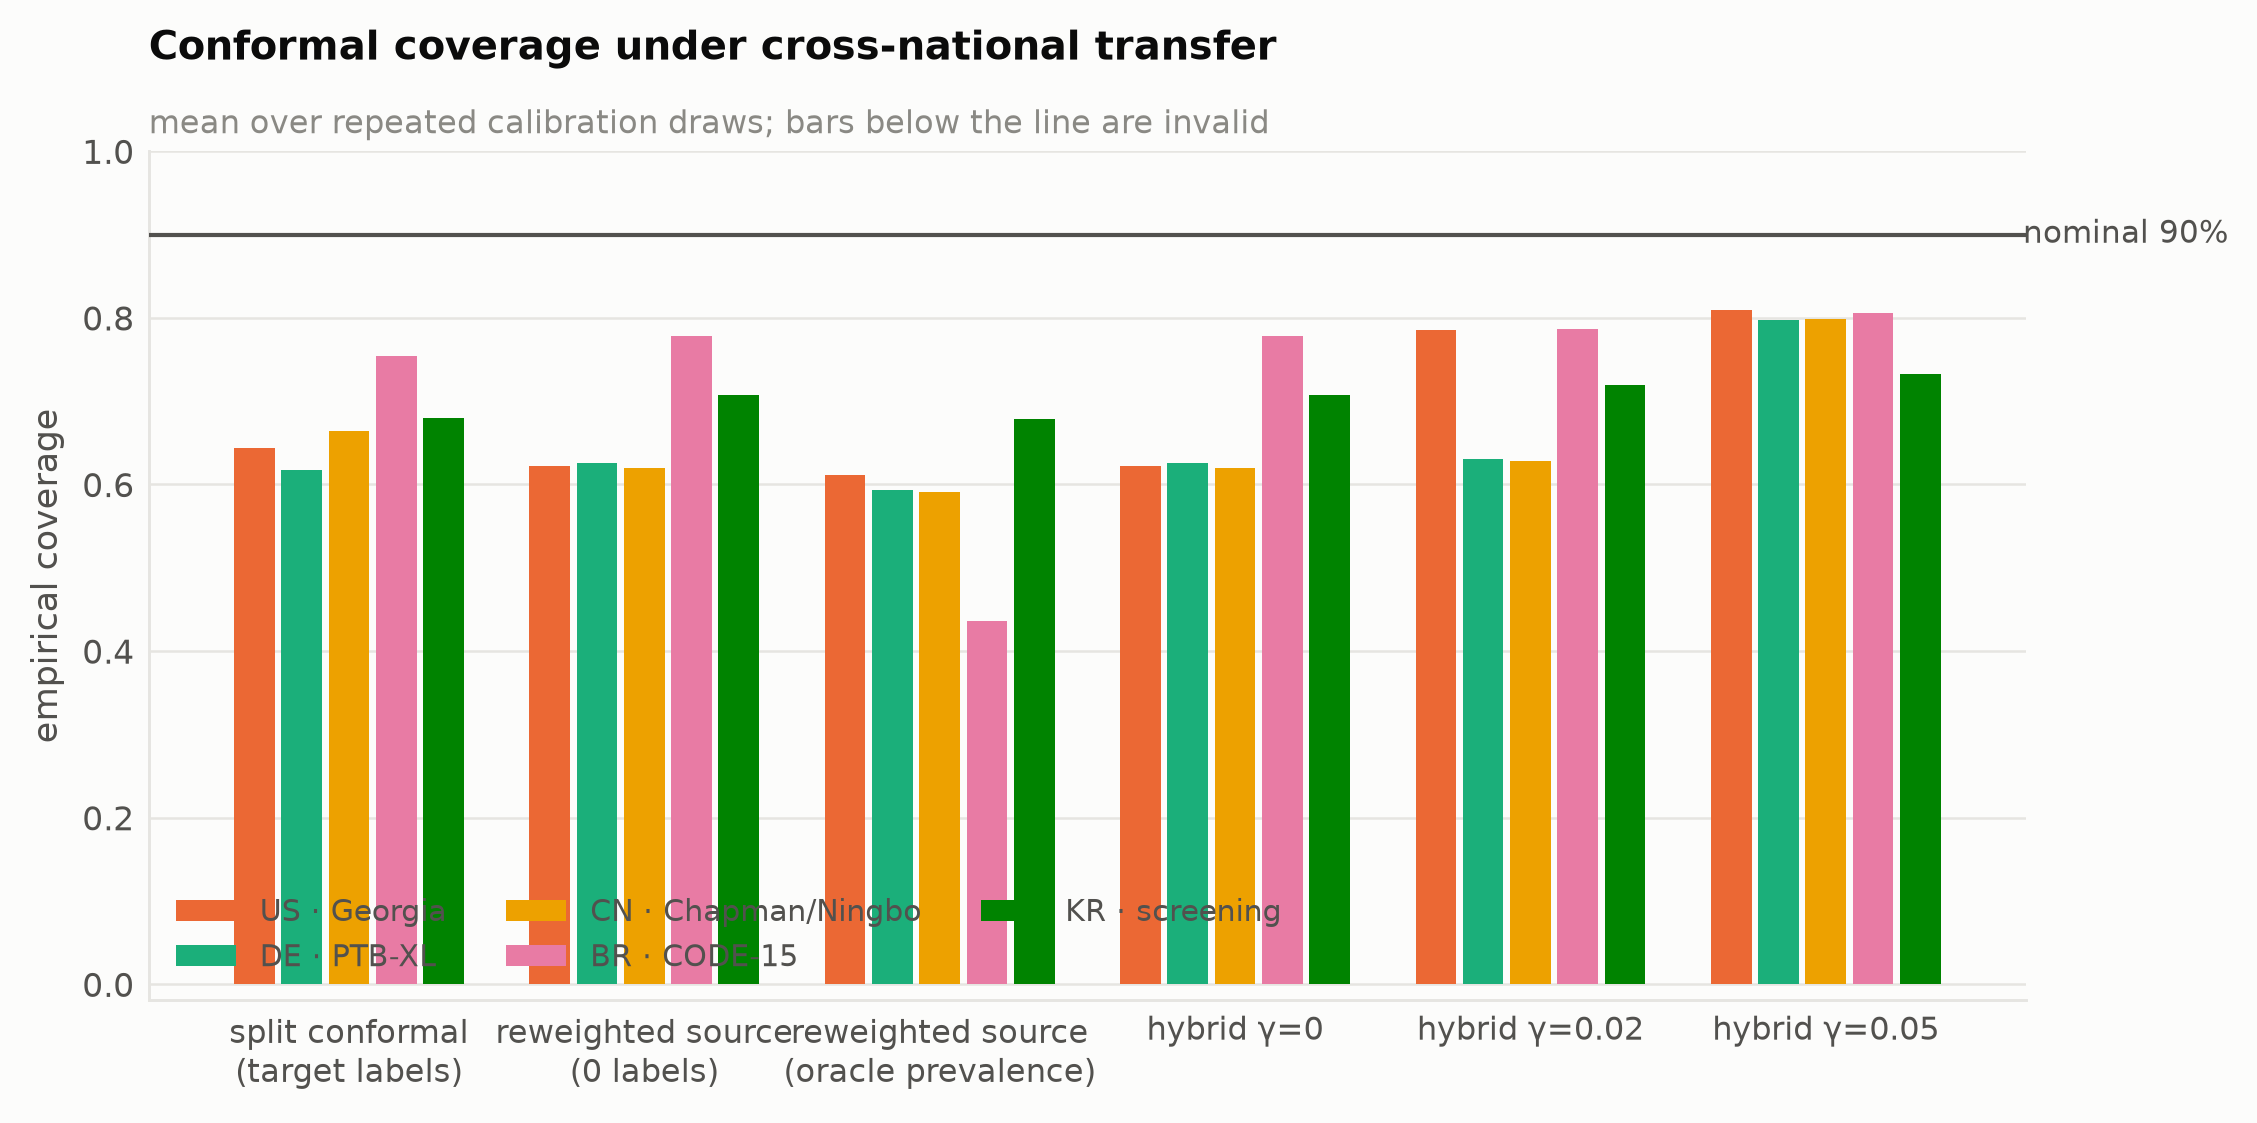
\includegraphics[width=\textwidth]{figures/fig6_conformal.pdf}
\caption{Coverage by procedure and site, averaged over repeated calibration
draws.  Bars below the rule are invalid.}
\label{fig:conformal}
\end{figure}

\subsection{The collapse map}

Figure~\ref{fig:collapse} summarises both halves of the result by site and
label: how far calibration falls, and how much of that fall one
correctly measured number would repair.  It is the object we propose as the
deployment artefact --- not a single external-validation AUROC, but a statement
per site and per label of how much the probabilities move and how much of that
movement one measured number would undo.

\begin{figure}[t]\centering
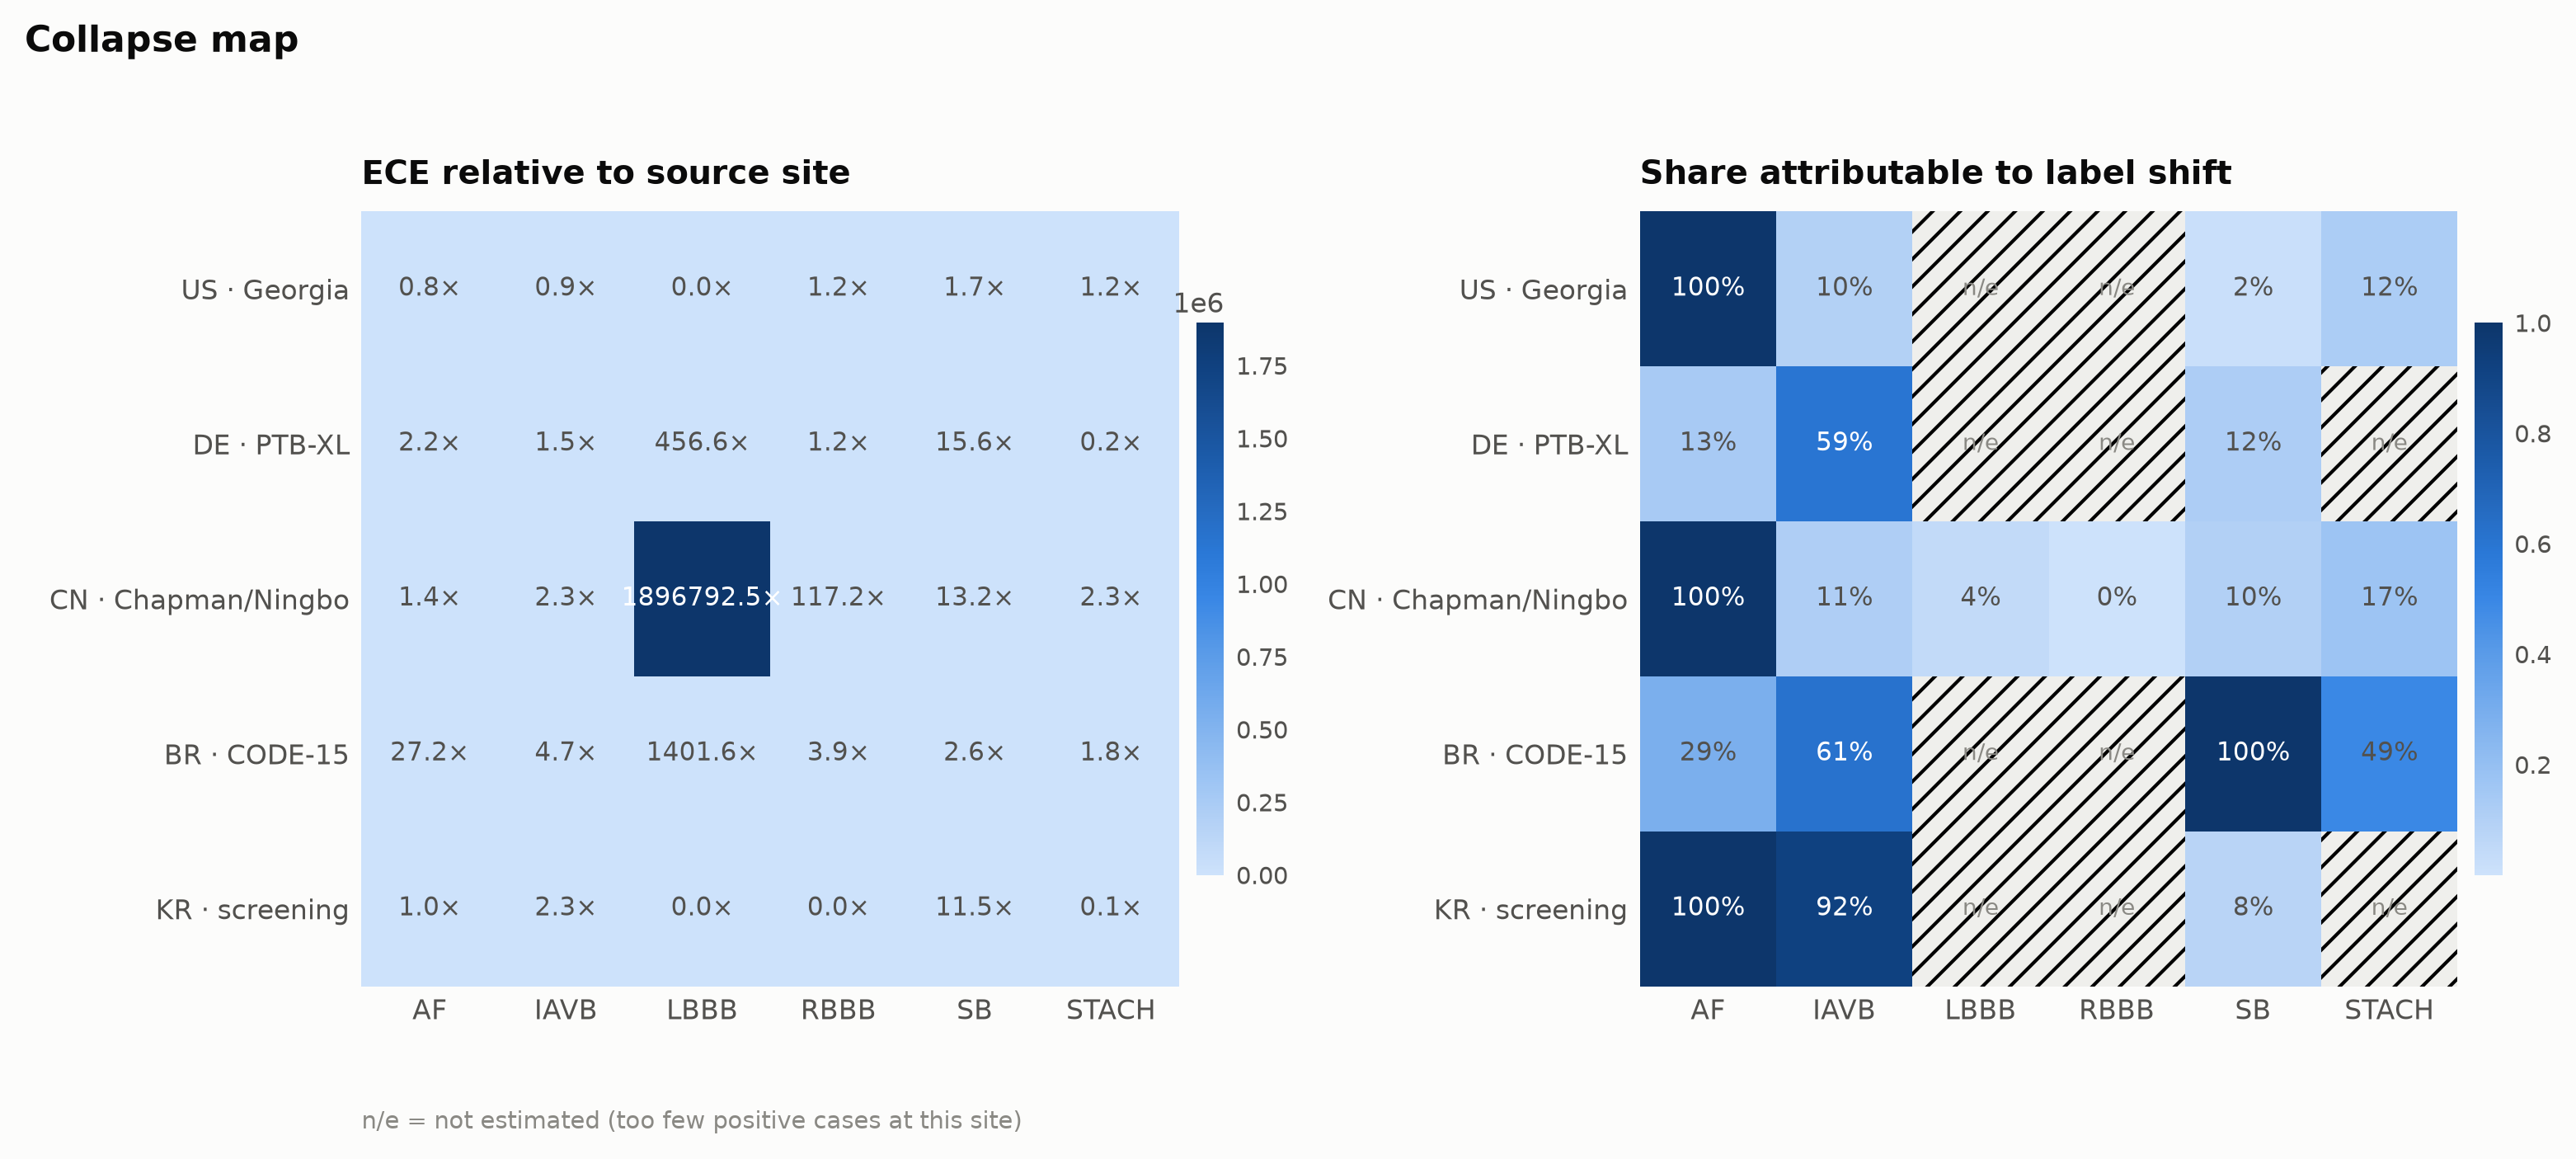
\includegraphics[width=\textwidth]{figures/fig5_collapse_map.pdf}
\caption{Collapse map. Left: ECE relative to the source site. Right: the share
attributable to label shift --- what one correctly measured number would repair.
Single-hue ramps, direct-labelled so the figure survives greyscale printing.}
\label{fig:collapse}
\end{figure}
